% This must be in the first 5 lines to tell arXiv to use pdfLaTeX, which is strongly recommended.
\pdfoutput=1
% In particular, the hyperref package requires pdfLaTeX in order to break URLs across lines.

\documentclass[11pt]{article}

\usepackage[a4paper, total={6in, 8in}]{geometry}
\usepackage{lineno}
\linenumbers

\usepackage{caption,subcaption}

\usepackage{mystyle}

\usetikzlibrary{calc,patterns,angles,quotes}    
\usetikzlibrary{decorations.pathmorphing}
\tikzset{snake it/.style={decorate, decoration=snake}}

\usepackage{natbib}
\bibliographystyle{abbrvnat}
\usepackage{hyperref}

% Standard package includes
\usepackage{times}
\usepackage{latexsym}

% For proper rendering and hyphenation of words containing Latin characters (including in bib files)
\usepackage[T1]{fontenc}
% For Vietnamese characters
% \usepackage[T5]{fontenc}
% See https://www.latex-project.org/help/documentation/encguide.pdf for other character sets

% This assumes your files are encoded as UTF8
\usepackage[utf8]{inputenc}


\title{Learning to Augment: Non-Autoregressive Translation}

\author{Justin Chiu \\
  Cornell Tech \\
  \texttt{jtc257@cornell.edu}}

\begin{document}
\maketitle
\begin{abstract}
Abstract
\end{abstract}

\section{Introduction}
Learned models of data are often misspecified.
When the goal of modeling is not density estimation,
but some alternative objective, this misspecification may lead to undesirable
behaviour under the maximum likelihood objective.
In this note, we consider learned data augmentation techniques to edit
each data point so that the augmented data is more amenable to a particular model class,
while hopefully preserving the properties we care about.

A concrete example of a setup where maximum likelihood may not be desirable is
non-autoregressive translation, which we focus on in this note.
In translation, the goal is to translate a source sentence from one language
into a sentence in a different target language.
The success of translation is measured by the BLEU score
between our generated translation and the true reference target sentence.
As the BLEU score is not a function of distributional closeness to the true data,
translation systems often discard distributional information and
output a single translation of a source sentence.
However, the training objective is still often maximum likelihood, a function of
the model distribution.

In the case of non-autoregressive translation, this results in undesirable behaviour.
As non-autoregressive models cannot model output dependencies,
resulting models trained via maximum likelihood using the true distribution
often have pathological errors due to misspecification,
and therefore poor BLEU scores.
We aim to resolve this via data augmentation.

Prior work shows that distillation is a successful data augmentation approach.
We instead rely on neural editor models \citep{edit},
which are a trainable alternative to data augmentation \citep{recombine}.

\section{Problem Setup}
Source sentence $x$, target sentence $y$.
True translation distribution $p(y \mid x)$.

We propose to, given a family of student models $q_\theta(y \mid x)$,
learn an edit model $q_\phi(\hat{y} \mid y, x)$ whose conditional distribution over $\hat{y}$
is easier for the student model $q_\theta$ to learn.
Learning an intermediate distribution will allow the student model to focus on only modeling
the important aspects of the true distribution.

To accomplish this, we propose to solve the following optimization problem
\begin{equation}
    \label{eqn:outer}
    \argmin_\phi \KL{p(y \mid x) || \sum_y q_\phi(\hat{y} \mid y, x)p(y \mid x)}
    + \min_\theta \KL{q_\phi(\hat{y} \mid y, x) || q_\theta(\hat{y} \mid x)}.
\end{equation}
This is a bilevel optimization problem, where we want to find the edit model
that is able to balance faithfulness to the true data (the first term)
as well as learnability of the student model (the second term).
We refer to Equation \ref{eqn:outer} as the outer problem,
and the second term as the inner problem:
\begin{equation}
    \label{eqn:inner}
    \argmin_\theta \KL{q_\phi(\hat{y} \mid y, x) || q_\theta(\hat{y} \mid x)}.
\end{equation}
The first term of the outer problem, the KL divergence between the true distribution
and the marginal posterior of the edit distribution,
serves as a regularizer and encourages the marginal distribution of
the edit distribution combined with the data distribution to be close to the
original data distribution.
As this setting may be both too restrictive as well as not example-specific,
we also consider the following variation:
\begin{equation}
    \label{eqn:regularized-bilevel}
    \argmin_\phi \sum_y \Omega(y, q_\phi(\hat{y} \mid y, x))
    + \min_\theta \KL{q_\phi(\hat{y} \mid y, x) || q_\theta(\hat{y} \mid x)},
\end{equation}
allowing us to perform instance-level regularization rather than distributional.

\section{Method 1: The Exact Setting}
We first make the simplifying assumption that we can solve the inner problem exactly.
In order to then solve the full outer problem, we will differentiate through the solution of the
inner problem.
In full generality, this would require an application of the implicit function theorem,
or approximations through sampling or incomplete optimization.

\subsection{Experiment: Length-2 Binary Strings + Non-autoregressive Student}
Our first experiment will determine whether training an edit model is possible in a
very simple setting, where we can compute the solution to the inner problem
(training the student model given an edit model) in closed form,
and subsequently differentiate through that procedure.

We restrict our attention to distributions over target sentences that are
binary strings of length 2 without conditioning on a source sentence.
In particular, our true distribution takes the form
$$y = b_1\cdot 00 + b_2\cdot 01 + b_3\cdot 10 + b_4\cdot 11,$$
where $b\sim\Cat(\lambda)$, represented as a one-hot sample
(meaning only one of $b_i$ can be 1, while the rest must be 0).
As we are interested in disambiguation, we first focus on the case where
$b_1, b_4 \approx 0$, and $b_2 < b_3$.
The edit model then takes the form
$$q_\phi(\hat{y} \mid y)= [\phi]_{\hat{y},y},$$
where $\hat{y},y \in \set{0,1}^2 = \mcY$ and $\phi \in [0,1]^{\mcY\times\mcY}$.
The student is nonautoregressive, and has the form
$$q_\theta(\hat{y}) = \prod_t q_\theta(\hat{y}_t)
= [\theta]_{1,\hat{y}_1} \cdot [\theta]_{2,\hat{y}_2},$$
where $\theta\in[0,1]^{2\times\mcY}$.

In this setting, we can exactly compute the solution of the inner problem,
$$
\argmin_\theta \Es{y}{\KL{q_\phi(\hat{y} \mid y)} || q_\theta(\hat{y})}
= \argmin_\theta \Es{y}{\sum_{\hat{y}} q_\phi(\hat{y} \mid y)
    \left(\log q_\phi(\hat{y} \mid y) - \log q_\theta(\hat{y})\right)
},
$$
and differentiate through it.
The minimizer is given by
\begin{align*}
    [\theta]_{1,0} &= \sum_y\sum_{\hat{y}} p(y)q_\phi(\hat{y}\mid y) 1(\hat{y}_1=0)\\
    [\theta]_{2,0} &= \sum_y\sum_{\hat{y}} p(y)q_\phi(\hat{y}\mid y) 1(\hat{y}_2=0)\\
    [\theta]_{t,1} &= 1 - [\theta]_{t,0},
\end{align*}
which is differentiable wrt $\phi$.

\paragraph{Results}
We find that the editor model is able to disambiguate the true data
and produces a new data distribution with no dependencies across time,
resulting in a distribution that is easier for the student to match.
We see the results of training the editor model with the following conditions:
\begin{itemize}
    \item $b = [0.001, 0.45, 0.54, 0.001]$
    \item Editor is initialized to uniform everywhere except
        the transitions from [0,1] and [1,0], where transitions to
        [0,0] and [1,1] are given low mass in order to speed up training
    \item We recompute the parameters of the student by
        solving the inner problem at every iteration
    \item We solve the outer problem via gradient descent
        (1k iterations, learning rate of 1e-3)
\end{itemize}
We see in Figure \ref{fig:editor-toy} (right) that the editor learns to
bias the data further towards $[1,0]$.
This results in the student model being very certain, as seen in Figure
\ref{fig:student-toy} (right).
In this very simple setting, the bilevel optimization formulation
successfully increases the assymmetry of the data.

\begin{figure}[h]
\centering
\begin{subfigure}[t]{0.45\textwidth}
\centering
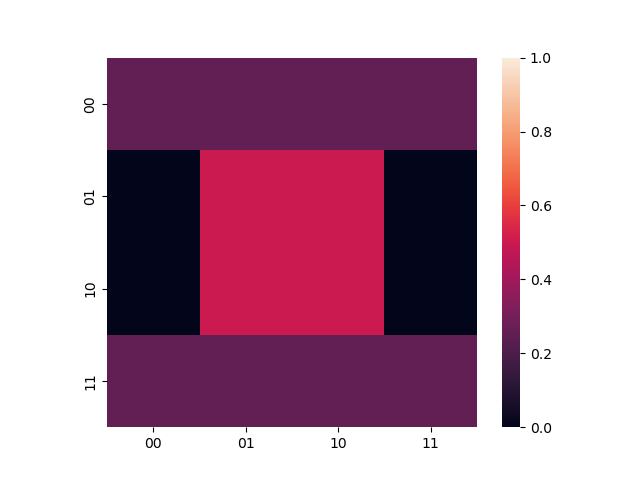
\includegraphics[height=2in]{../plots/very_uneven_prior_editor_init.png}
\end{subfigure}
\begin{subfigure}[t]{0.45\textwidth}
\centering
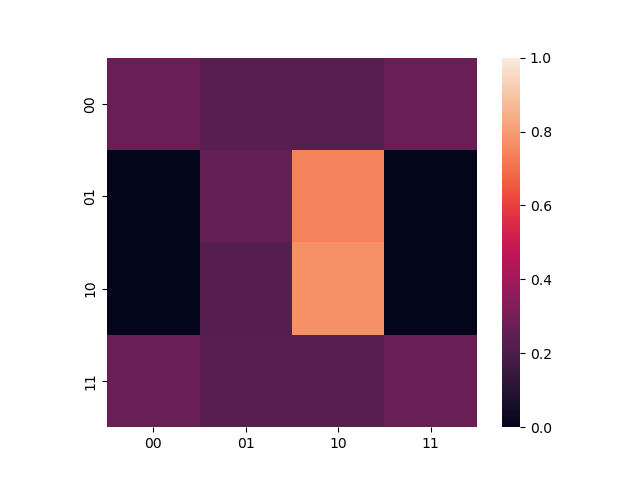
\includegraphics[height=2in]{../plots/very_uneven_prior_editor_final.png}
\end{subfigure}
\caption{
\label{fig:editor-toy}
The emission probabilities for the editor model at the start of training (left)
and end of training (right).
}
\end{figure}

\begin{figure}[h]
\centering
\begin{subfigure}[t]{0.45\textwidth}
\centering
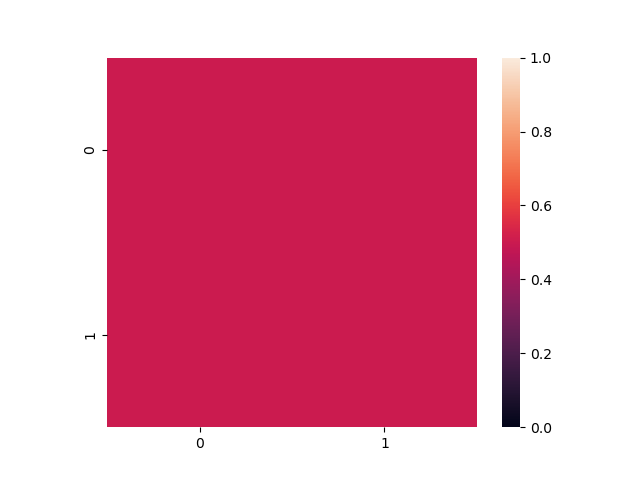
\includegraphics[height=2in]{../plots/very_uneven_prior_student_init.png}
\end{subfigure}
\begin{subfigure}[t]{0.45\textwidth}
\centering
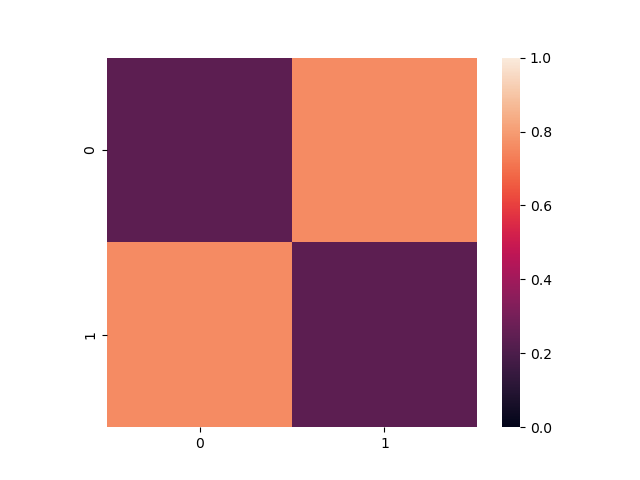
\includegraphics[height=2in]{../plots/very_uneven_prior_student_final.png}
\end{subfigure}
\caption{
\label{fig:student-toy}
The emission probabilities for the student model at the start of training (left)
and end of training (right).
}
\end{figure}

However, in settings where the true data distribution is less skewed,
the objective does not allow the edit model to deviate too far.
Figures \ref{fig:editor-toy2} and \ref{fig:student-toy2} show the results
when $b = [1e-3, 0.5, 0.5, 1-e3]$.
In this setting, both the data distribution and edit distribution are symmetric,
resulting in the student remaining at a standstill.
This is because any movement away from the true distribution would incur
too large a penalty in the first term of the objective,
$\KL{p(y) || \sum_y q(\hat{y} \mid y)p(y)}$.

\begin{figure}[h]
\centering
\begin{subfigure}[t]{0.45\textwidth}
\centering
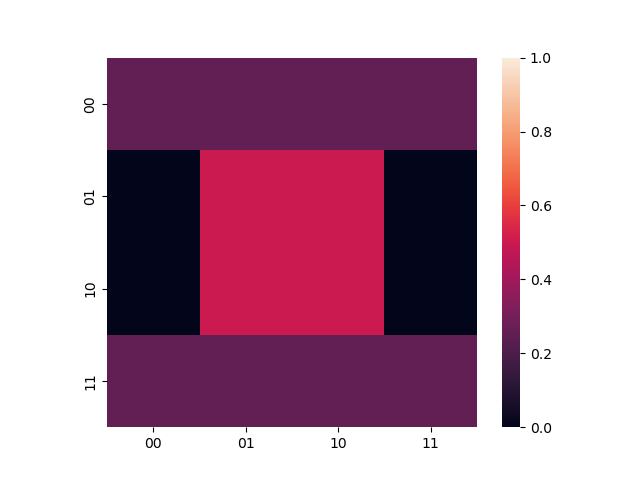
\includegraphics[height=2in]{../plots/even_prior_editor_init.png}
\end{subfigure}
\begin{subfigure}[t]{0.45\textwidth}
\centering
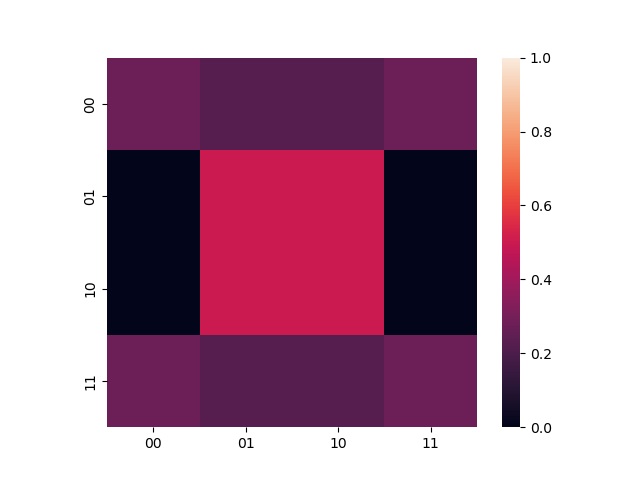
\includegraphics[height=2in]{../plots/even_prior_editor_final.png}
\end{subfigure}
\caption{
\label{fig:editor-toy2}
The emission probabilities for the editor model at the start of training (left)
and end of training (right) with an even true data distribution.
}
\end{figure}

\begin{figure}[h]
\centering
\begin{subfigure}[t]{0.45\textwidth}
\centering
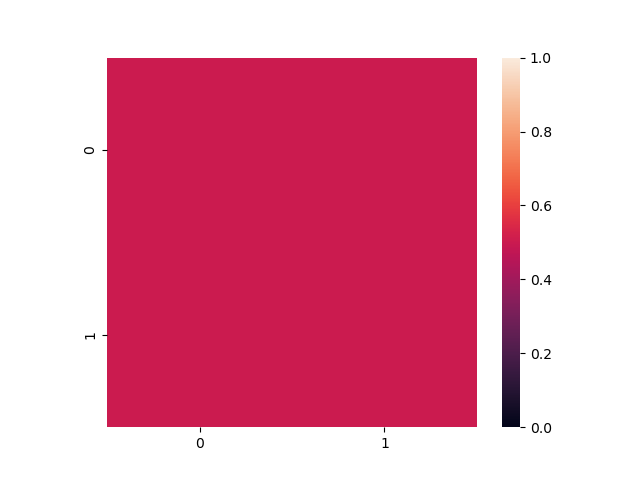
\includegraphics[height=2in]{../plots/even_prior_student_init.png}
\end{subfigure}
\begin{subfigure}[t]{0.45\textwidth}
\centering
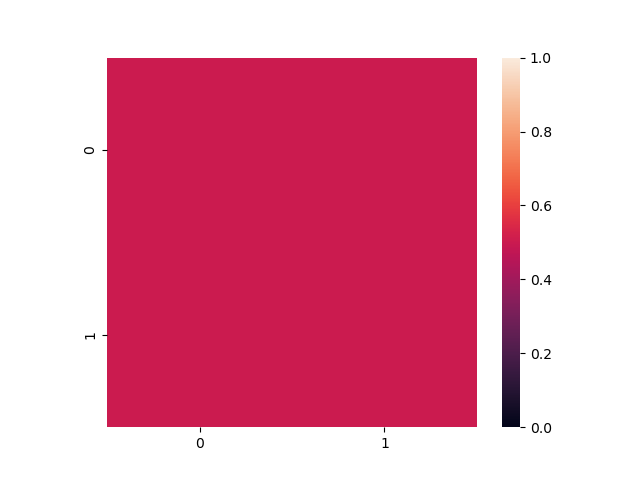
\includegraphics[height=2in]{../plots/even_prior_student_final.png}
\end{subfigure}
\caption{
\label{fig:student-toy2}
The emission probabilities for the student model at the start of training (left)
and end of training (right) with an even true data distribution.
}
\end{figure}



\section*{Decoding: work back into problem setup later}
Given data consisting of $(x,y)$ pairs, our goal is to learn a model $q_\theta(y \mid x)$
such that it maximizes the functional
\begin{equation}
    \label{eqn:obj}
    F(q) = \Es{p(x,y)}{\argmax_{\hat{y}}d(q_\theta(\hat{y} \mid x), y)},
\end{equation}
where $p(x,y)$ is the data distribution and $d$ is some measure of correctness between our
prediction $\hat{y}$ and the true output $y$.

\bibliography{bib}

\end{document}
